\chapter{Supporting Information for Reproducibility Study}
\label{chap:rep_SI}

%---------------------------------------------
\newpage % NOTE: The appendix title should be on its own page.
%---------------------------------------------



\section{Forcefield parameters}
\begin{table}
\caption{Non-bonded parameters for SPC/E water} \label{tab:water}
\centering
\begin{tabular}{lcccc}
   & epsilon (kJ/mol) & sigma (nm) & charge (e) & mass (amu) \\ \hline
OW & 0.650194         & 0.316557   & -0.8476    &  15.99940  \\ 
HW & 0.0              & 0.0        &  0.4238    &  1.00800   \\ \hline
\end{tabular}
\end{table}

\begin{table}
\caption{Non-bonded parameters for TraPPE-UA benzene} \label{tab:bz_nonbond}
\centering
\begin{tabular}{lccc}
    & epsilon (kJ/mol)  & sigma (nm) & mass (amu) \\ \hline
CHE & 0.419880362216737 & 0.3695     &  13.01900  \\ \hline
\end{tabular}
\end{table}

\section{Potential energy plots}
\begin{figure}[h!]
    \centering
    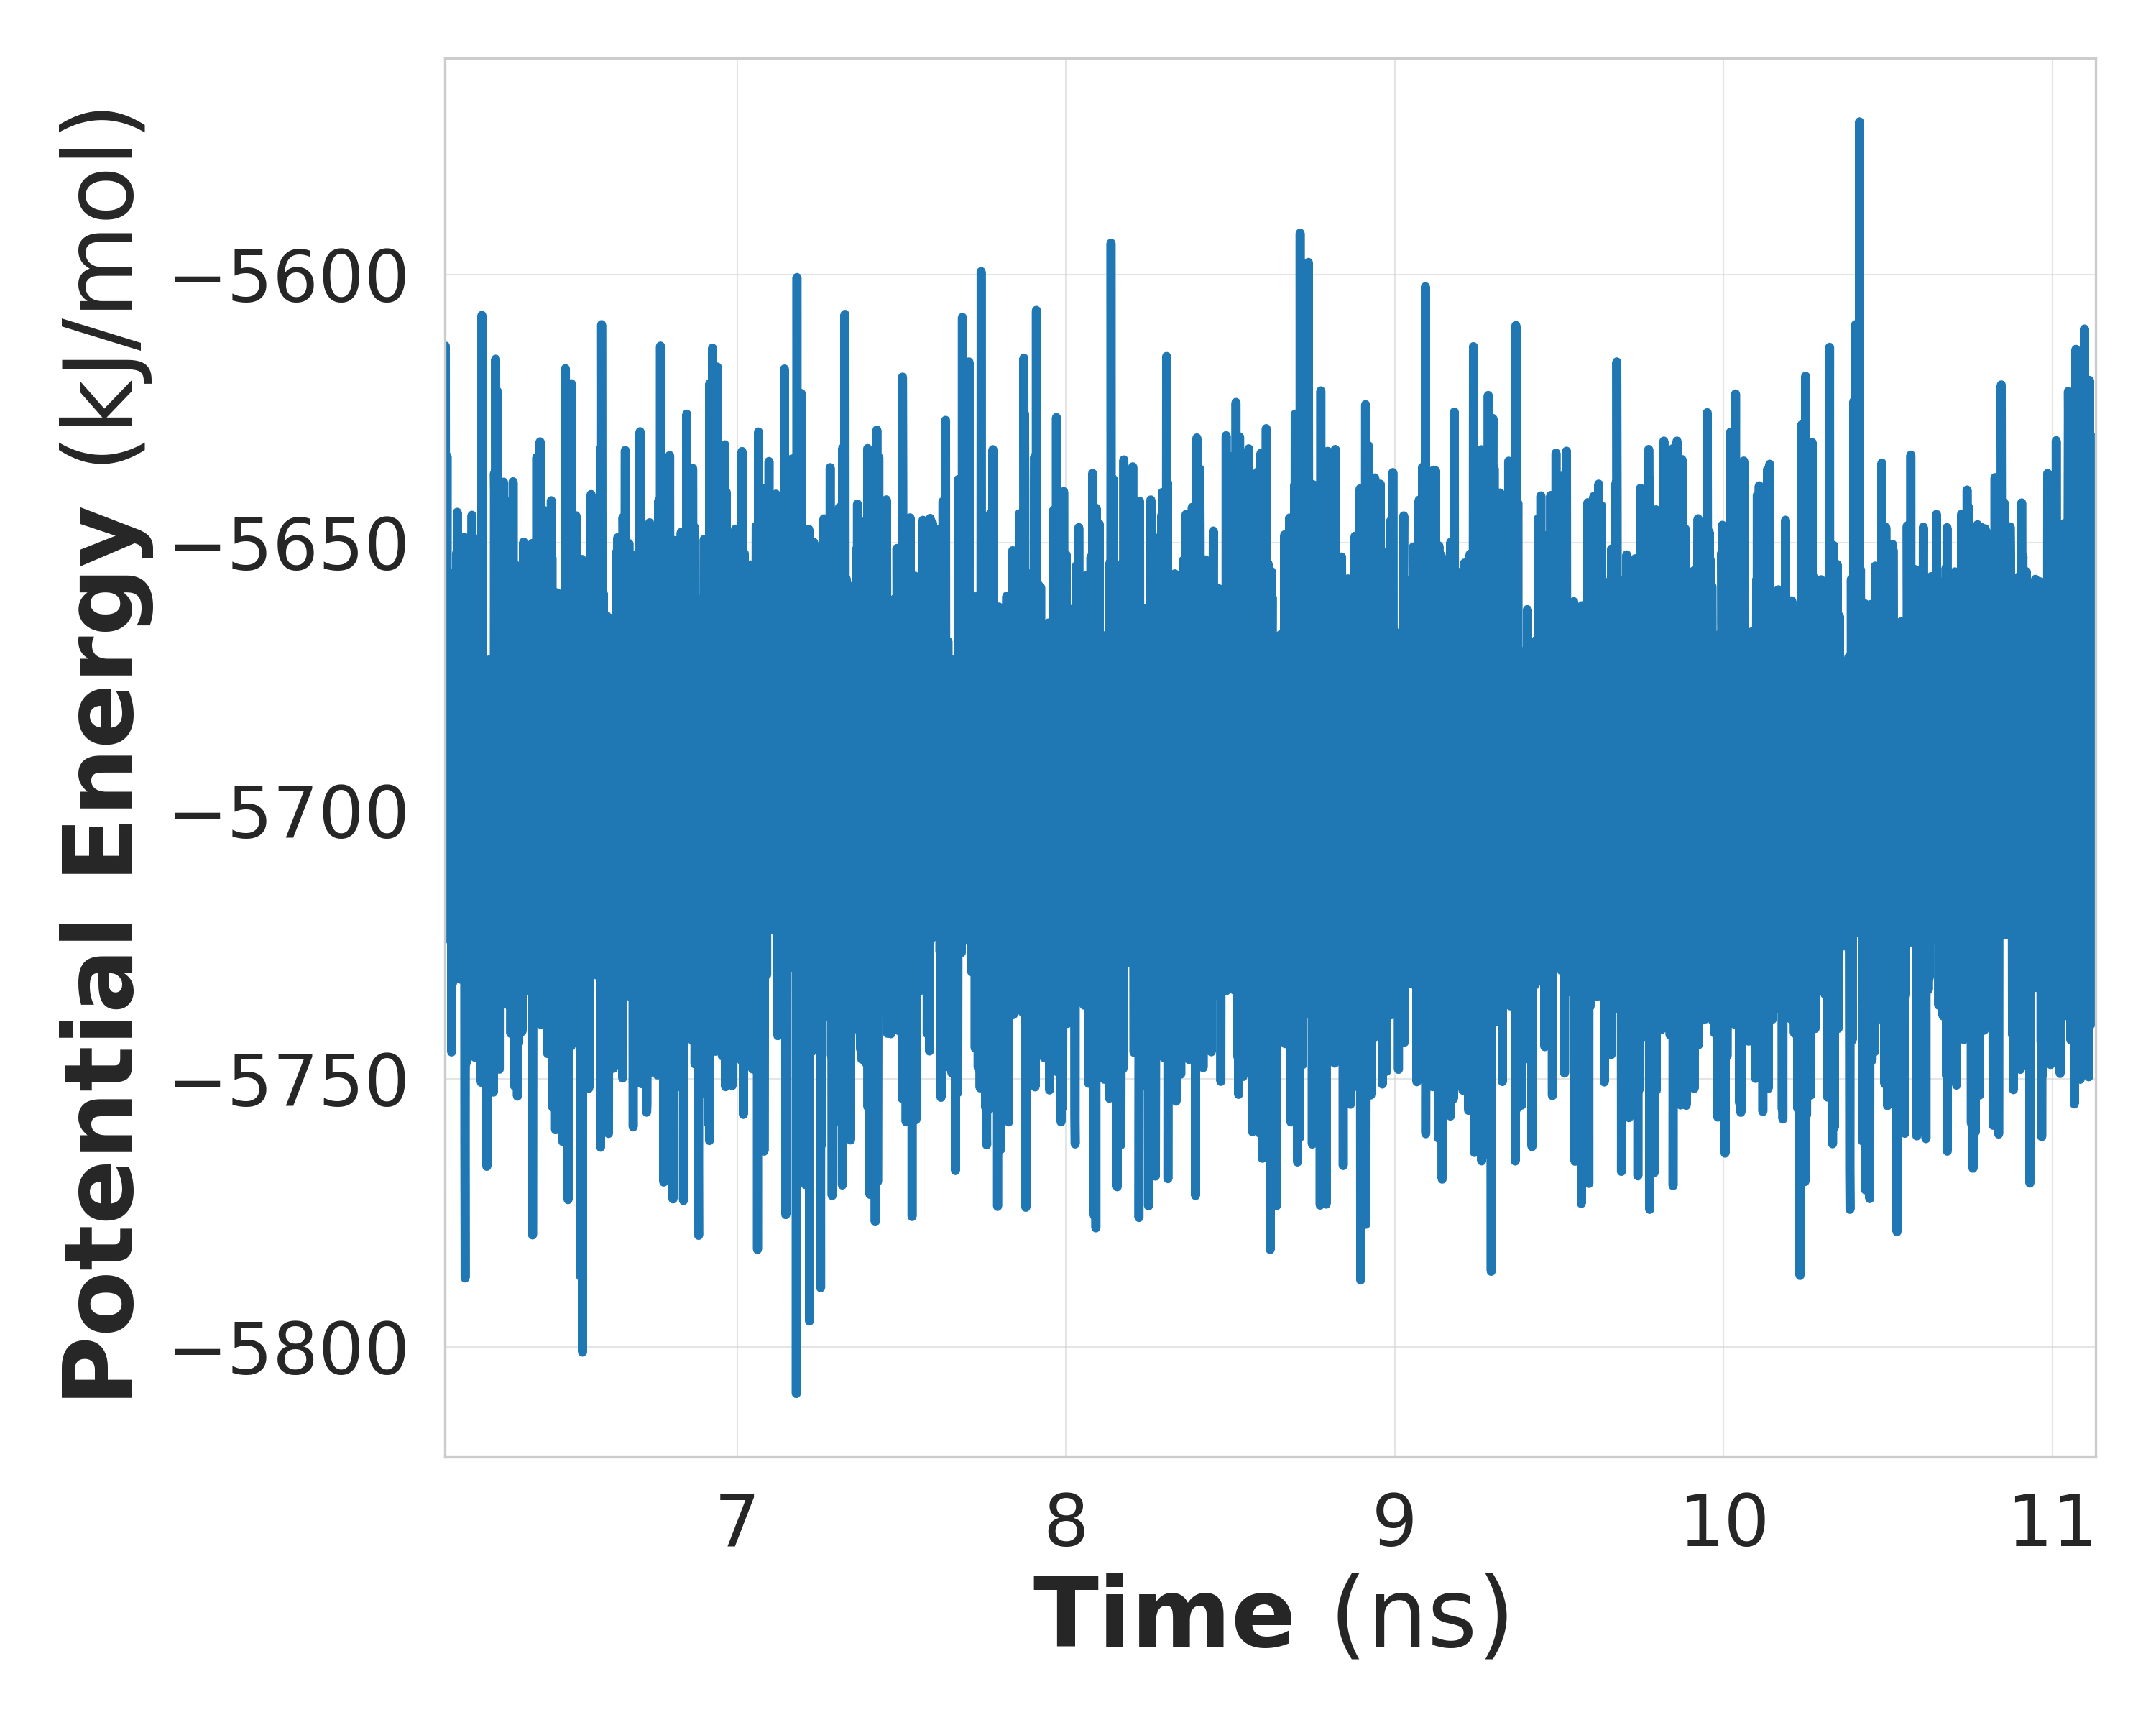
\includegraphics[width=0.8\linewidth,keepaspectratio]{figures/rep_study/methane_pe.png}
    \caption{Potential energy over time for methaneUA NVT ensemble.}\label{fig:methane_pe_evolution}
\end{figure}

\begin{figure}[h!]
    \centering
    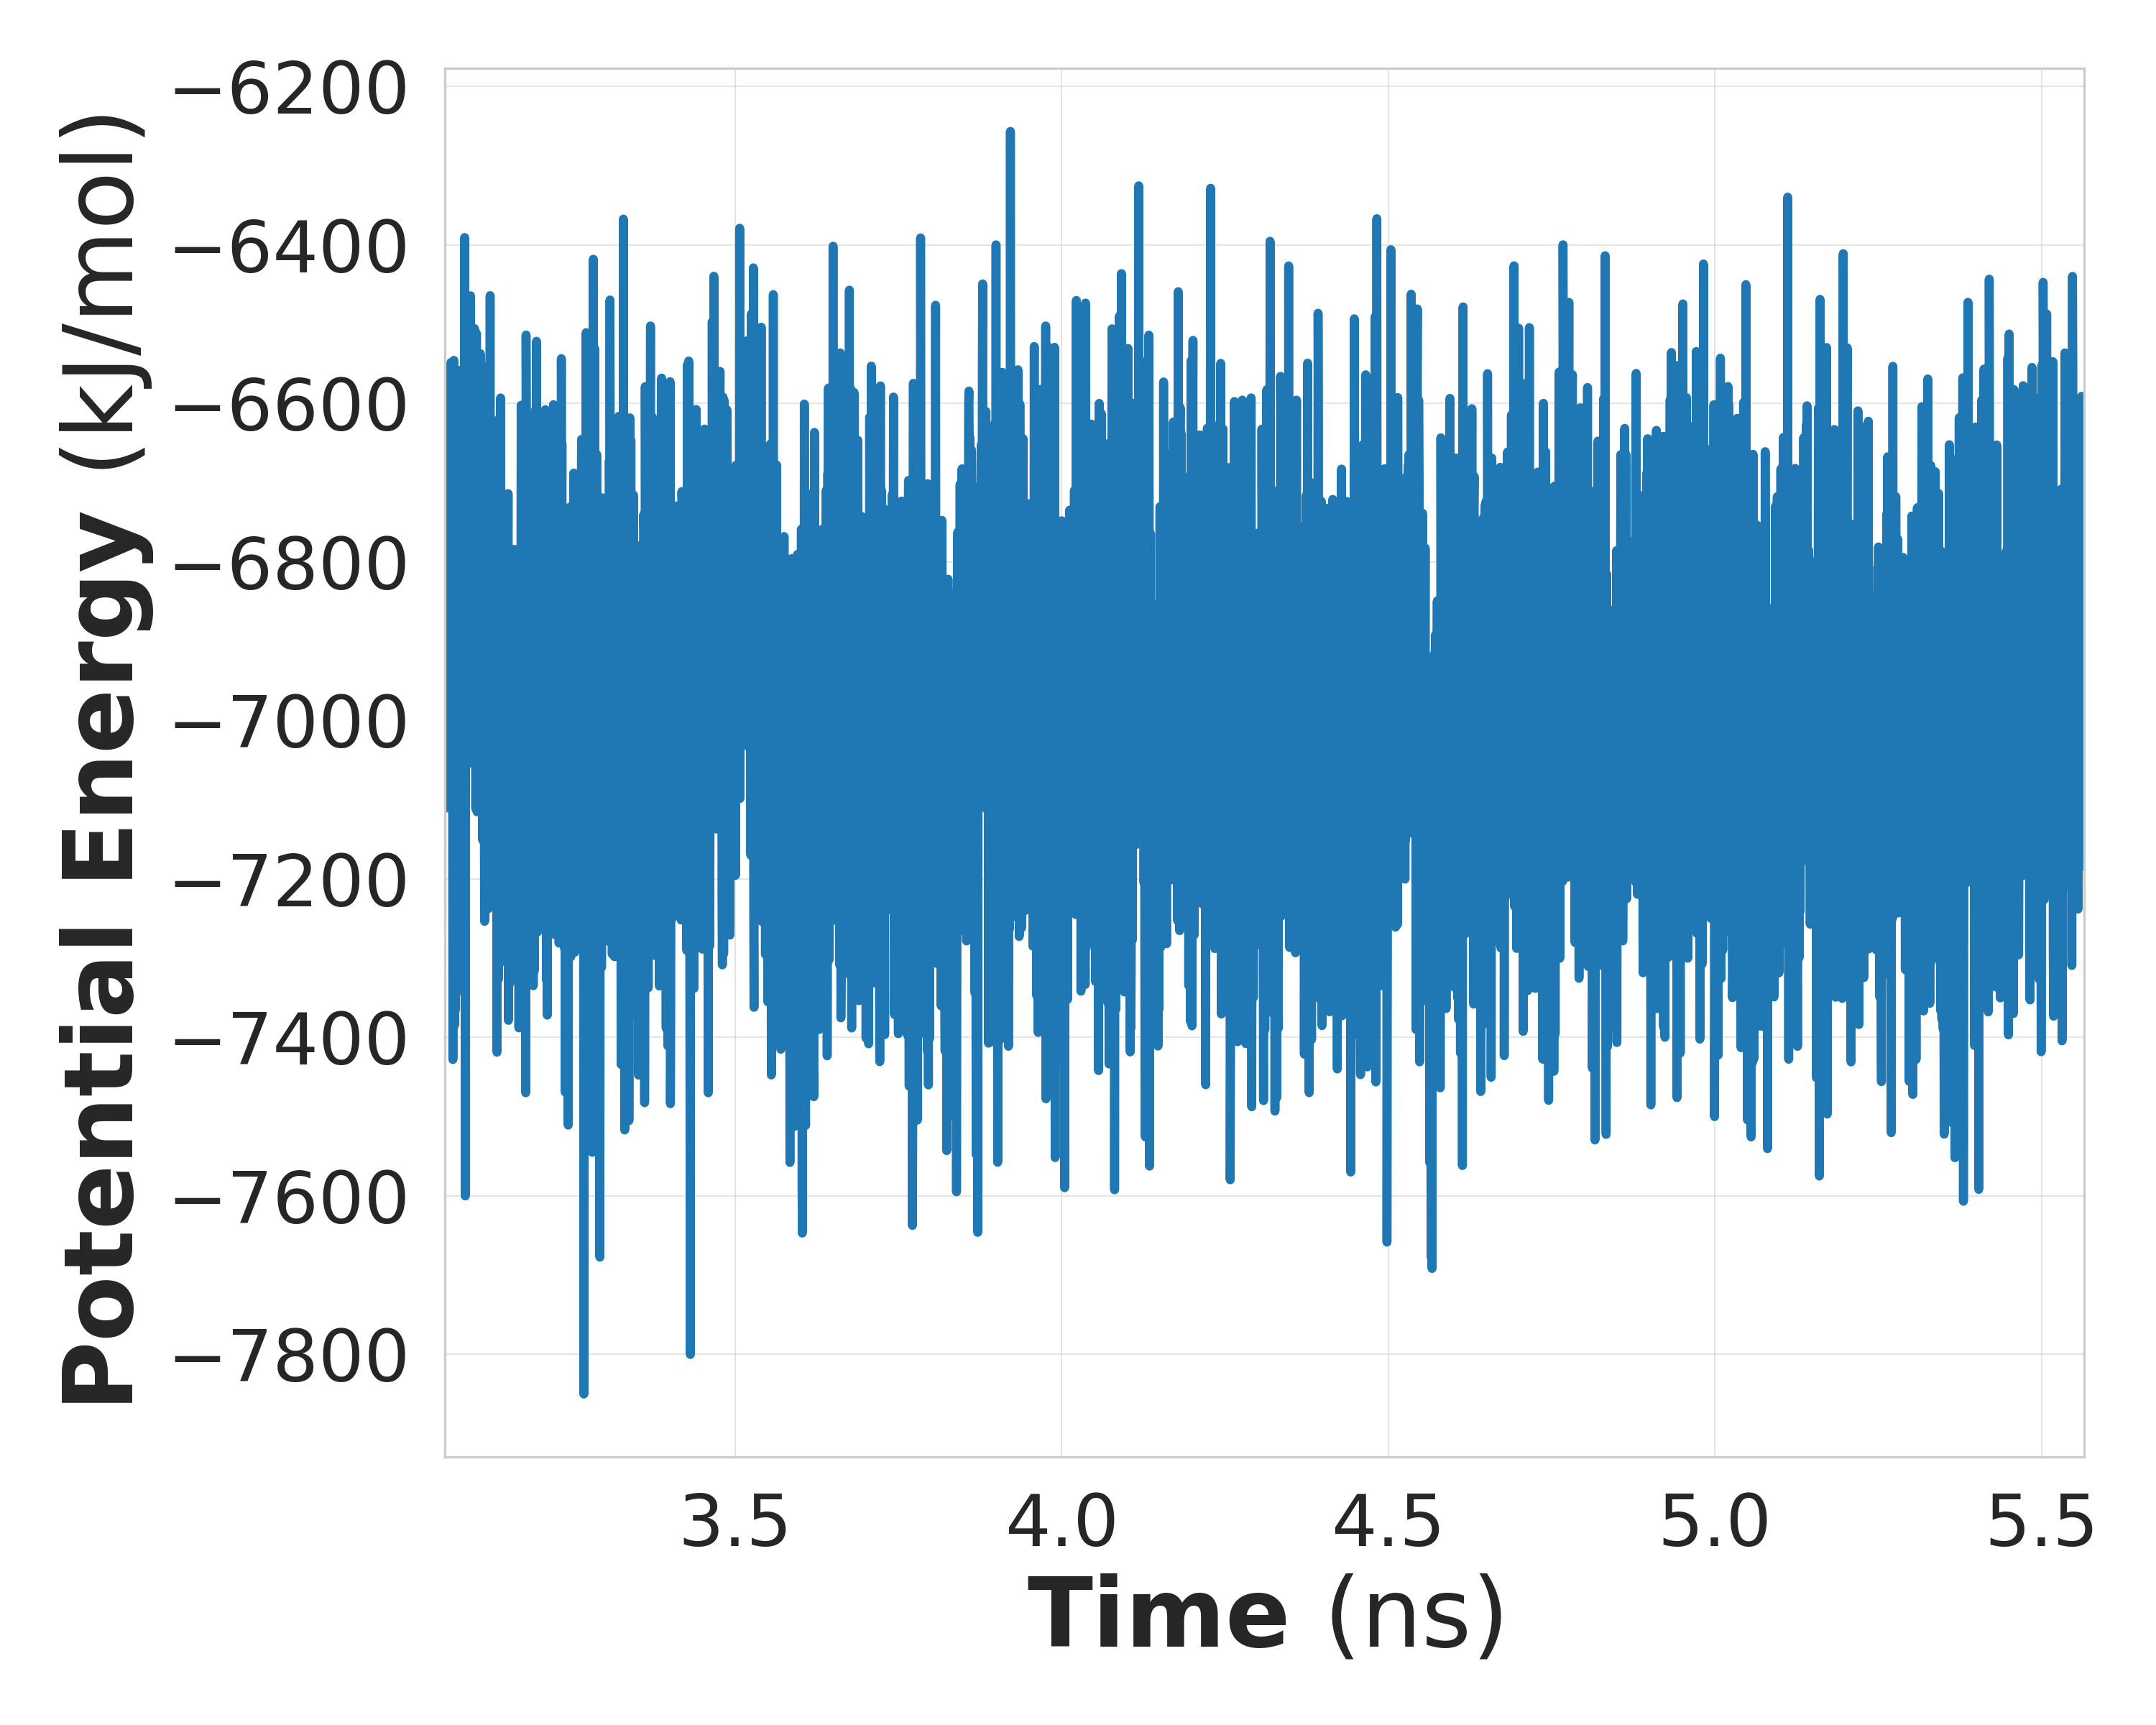
\includegraphics[width=0.8\linewidth,keepaspectratio]{figures/rep_study/ethanol_pe.png}
    \caption{Potential energy over time for ethanolAA NVT ensemble.}\label{fig:ethanol_pe_evolution}
\end{figure}

\section{Single-point Energies}

\begin{table}
\caption{Single-point energy breakdown for methaneUA}\label{tab:sp_methane}
\centering
\begin{tabular}{rccc}
Engine & Potential & VDW & Tail Correction \\ \hline
LAMMPS-VU & 5.367E+05 & 5.37E+05 & -1.28E+02 \\
LAMMPS-UD & 5.369E+05 & 5.37E+05 & -1.19E+02 \\
MCCCS & 5.367E+05 & 5.37E+05 & -1.28E+02 \\
HOOMD & 5.368E+05 & 5.37E+05 & -1.19E+02 \\
GROMACS & 5.368E+05 & 5.37E+05 & -1.19E+02 \\
GOMC & 5.367E+05 & - & -1.28E+02 \\
Cassandra & 5.367E+05 & 5.37E+05 & -1.28E+02 \\ \hline
\end{tabular}
\end{table}

\begin{table}
\caption{Single-point energy breakdown for pentaneUA}\label{tab:sp_pentane}
\centering
\begin{tabular}{rcccccc}
\hline
Engine & Potential & VDW & Tail Correction & Bond & Angle & Dihedral \\ \hline
LAMMPS-VU & 5.377E+05 & 5.38E+05 & -1.81E+02 & 0 & 0 & 0 \\
LAMMPS-UD & 5.366E+05 & 5.37E+05 & -1.68E+02 & 5.50E-07 & 6.30E-08 & 2.90E-09 \\
MCCCS & 5.377E+05 & 5.38E+05 & -1.81E+02 & 0 & 0 & 0 \\
HOOMD & 5.378E+05 & 5.38E+05 & -1.68E+02 & 0 & 0 & 0 \\
GROMACS & 5.378E+05 & 5.38E+05 & -1.68E+02 & 0 & 0 & 1.00E-02 \\
GOMC & 5.377E+05 & - & -1.81E+02 & - & - & - \\
Cassandra & 5.377E+05 & 5.38E+05 & -1.81E+02 & 0 & 6.37E-08 & 2.94E-09 \\ \hline
\end{tabular}
\end{table}

\begin{table}
\caption{Single-point energy breakdown for benzeneUA}\label{tab:sp_benzene}
\centering
\begin{tabular}{rccc}
\hline
Engine & Potential & VDW & Tail Correction \\ \hline
LAMMPS-VU & 3.889E+05 & 3.89E+05 & -2.51E+02 \\
LAMMPS-UD & 3.890E+05 & 3.89E+05 & -2.34E+02 \\
MCCCS & 3.889E+05 & 3.89E+05 & -2.51E+02 \\
HOOMD & 3.891E+05 & 3.89E+05 & -2.34E+02 \\
GROMACS & 3.891E+05 & 3.89E+05 & -2.34E+02 \\
Cassandra & 3.889E+05 & 3.89E+05 & -2.51E+02 \\
GOMC & 3.889E+05 & - & -2.51E+02 \\ \hline
\end{tabular}
\end{table}

\begin{table}
\caption{Single-point energy breakdown for SPC/E water}\label{tab:sp_water}
\centering
\begin{tabular}{rcccccccc}
\hline
Engine & Potential & VDW & Tail Correction & Total Electrostatic & Short Range Electrostatic & Long Range Electrostatic & Bond & Angle \\ \hline
LAMMPS-VU & 5.718E+04 & 7.67E+04 & -2.76E+02 & -1.95E+04 & 2.93E+05 & -3.12E+05 & 0 & 0 \\
LAMMPS-UD* & 5.977E+04 & 7.68E+04 & -2.49E+02 & -1.70E+04 & 2.90E+05 & -3.07E+05 & 0 & 0 \\
MCCCS & 5.717E+04 & 7.67E+04 & -2.76E+02 & -1.95E+04 & - & - & 0 & 0 \\
HOOMD & 5.718E+04 & 7.67E+04 & -2.76E+02 & -1.43E+04 & -5.18E+03 & 5.72E+04 & 0 & 0 \\
GROMACS* & 5.977E+04 & 7.68E+04 & -2.50E+02 & -1.70E+04 & -2.37E+04 & 6.64E+03 & 0 & 0 \\
GOMC & 5.718E+04 & - & -2.76E+02 & - & - & - & - & - \\
Cassandra & 5.732E+04 & 7.68E+04 & -2.76E+02 & -1.95E+04 & 3.25E+05 & -3.44E+05 & 0 & 7.27E-09 \\ \hline
\multicolumn{4}{l}{\small *The discrepancies seen in LAMMPS-UD and GROMACS are most likely due to a different size simulation box.} \\
\end{tabular}
\end{table}

\begin{table}
\caption{Single-point energy breakdown for OPLSAA ethanol}\label{tab:sp_ethanol}
\centering
\begin{tabular}{rccccccccc}
Engine & Potential & VDW & Tail Correction & Total Electrostatic & Short Range Electrostatic & Long Range Electrostatic & Bond & Angle & Dihedral \\ \hline
LAMMPS-VU & 3.141E+04 & 1.94E+04 & -4.18E+02 & 3.58E+03 & 8.13E+04 & -7.77E+04 & 0 & 7.23E+03 & 1.19E+03 \\
LAMMPS-UD* & 3.153E+04 & 1.96E+04 & -3.83E+02 & 3.55E+03 & 8.06E+04 & -7.71E+04 & 5.96E-05 & 7.23E+03 & 1.19E+03 \\
MCCCS & 3.141E+04 & 1.94E+04 & -4.18E+02 & 3.58E+03 & - & - & 0 & 7.23E+03 & 1.19E+03 \\
HOOMD & 3.141E+04 & 1.94E+04 & -4.18E+02 & 2.31E+03 & 1.27E+03 & 2.30E+04 & 7.23E+03 & 1.19E+03 & 8.43E+03 \\
GROMACS* & 3.153E+04 & 1.96E+04 & -3.83E+02 & 3.55E+03 & 1.69E+04 & 1.39E+03 & 0 & 7.23E+03 & 1.19E+03 \\
GOMC & 3.141E+04 &  & -4.18E+02 & - & - & - & - & - & - \\
Cassandra & 3.141E+04 & 1.94E+04 & -4.18E+02 & 3.58E+03 & 9.56E+04 & -9.21E+04 & - & 7.23E+03 & 1.19E+03 \\ \hline
\multicolumn{4}{l}{\small *The discrepancies seen in LAMMPS-UD and GROMACS are most likely due to a different size simulation box.}
\end{tabular}
\end{table}
